\section{Gaussian Processes}
\framecard{\insertsection}

% \subsection{Recap}
% \begin{frame}{\insertsubsection}
%     \framesubtitle{Linear Regression} 

%     \textcolor{UniGold}{\textbf{What was done until here?}}
%     \begin{itemize}
%         \item We assumed that our targets $t$ were \textcolor{UniOrange}{\textbf{i.i.d.}} and given by $t = y(\mathbf{x}) + \varepsilon$, where $\varepsilon \sim \mathcal{N}(0,\beta)$.
%         \item Our model is given by $\mathbf{y}(\mathbf{x}) = \Phi^{\top} \mathbf{w}$, where $\Phi$ is the \textcolor{UniOrange}{\textbf{design matrix}}, and this caracterize our model as \textcolor{UniOrange}{\textbf{linear in parameters}}.
%         \item The \textcolor{UniOrange}{\textbf{design matrix}} was defined as $ \phi_{i,j} = \phi_i(\mathbf{x}_j)$.
%         \item The \textcolor{UniOrange}{\textbf{parameters}} were given by $\mathbf{w} = \left( \Phi^{\top} \Phi \right)^{-1}\Phi^{\top} \mathbf{t}$.
%         \item These \textcolor{UniOrange}{\textbf{parameters}} calculated at the minimum of the cost function are called \textcolor{UniOrange}{\textbf{maximum likelihood}}.
%     \end{itemize}
%     \begin{columns}
%         \begin{column}{0.5\linewidth}  
%         \begin{center}
%         \centering
%         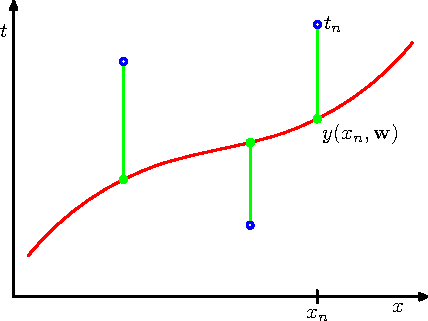
\includegraphics[width=0.9\linewidth]{Figure1c3.pdf}
%          \end{center}
%     \end{column}
%     \begin{column}{0.5\linewidth}  %%<--- here
%         \begin{figure}
%             \setlength\fwidth{0.07\textwidth}
%             \input{./codes/lnReg/"lnReg".tex}
%         \end{figure}
%     \end{column}
%     \end{columns}

% \end{frame}

% \begin{frame}{\insertsubsection}
%     \framesubtitle{Bayesian Linear Regression} 

%     \textcolor{UniGold}{\textbf{What was done until here?}}
%     \begin{itemize}
%         \item We put an \textcolor{UniOrange}{\textbf{uncertainty}} over the targets $t$ and the parameters $\mathbf{w}$.
%         \item We assumed that targets being \textcolor{UniOrange}{\textbf{distributed}} as $p( t| \mathbf{x}, \mathbf{w}, \beta) = \mathcal{N} ( t | y(\mathbf{x}, \mathbf{w}), \beta^{-1})$.
%         \item By \textcolor{UniOrange}{\textbf{Bayes' Rule}} we obtained that $p\left( \mathbf{w} | \mathbf{x}, \mathbf{t}, \alpha, \beta \right) \propto p\left(  \mathbf{t} |\mathbf{w} ,\mathbf{x}, \beta \right) p\left( \mathbf{w} | \alpha \right)$
%         \item This allowed to make an \textcolor{UniOrange}{\textbf{inference}} to obtain a \textcolor{UniOrange}{\textbf{prediction}} of the parameters in the \textcolor{UniOrange}{\textbf{weight-space}}.
        
%     \end{itemize}

%     % \begin{figure}
% 	% 	\label{fig:baReg}
%     %     \hspace*{-1.4cm}\includegraphics[totalheight=0.3\textheight]{./codes/baReg/"baReg".eps}
% 	% \end{figure}
% \end{frame}


% \begin{frame}{\insertsubsection}
%     \framesubtitle{A more clear way to se what is happening...} 

%     % \textcolor{UniGold}{\textbf{A more clear way to se what is happening...}}

%     % \begin{figure}
% 	% 	\label{fig:baReg}
%     %     \hspace*{-1.4cm}\includegraphics[totalheight=0.3\textheight]{"baRegInfII".eps}
% 	% \end{figure}
% \end{frame}

% %%%%%%%%%%%%%%%%%%%%%%%%%%%%%%%%%%%%%%%%%%%%%%%%%%%%%%%%%%%%%%%%%%%%%%%%%%%%%%%%%%%%%%%%%%%%%

% \begin{frame}{\insertsubsection}
%     \framesubtitle{Introducing kernels}

%     \textcolor{UniGold}{\textbf{What is kernel?}}
%     \begin{equation*}
%         \begin{aligned} f_{*} | \mathbf{x}_{*}, \Phi, \mathbf{t} & \sim \mathcal{N}\left(\boldsymbol{\phi}_{*}^{\top} \mathbf{S}_0 \Phi\left(K+\beta^{-2} I\right)^{-1} \mathbf{t}, \boldsymbol{\phi}_{*}^{\top} \mathbf{S}_0 \boldsymbol{\phi}_{*}-\boldsymbol{\phi}_{*}^{\top} \mathbf{S}_0 \Phi\left(K+\beta^{-2} I\right)^{-1} \Phi^{\top} \mathbf{S}_0 \boldsymbol{\phi}_{*}\right)
%         \end{aligned}
%     \end{equation*}

%     \begin{itemize}
%         \item We could observe the appearance of terms like $\Phi^{\top} \mathbf{S}_0 \Phi, \boldsymbol{\phi}_{*}^{\top} \mathbf{S}_0 \Phi, \text { or } \boldsymbol{\phi}_{*}^{\top} \mathbf{S}_0 \boldsymbol{\phi}_{*}$.
%         \item The common term between these operations is $k(\mathbf{x},\mathbf{x^{\prime}}) = \boldsymbol{\phi}(\mathbf{x})^{\top} \mathbf{S}_0 \boldsymbol{\phi}\left(\mathbf{x}^{\prime}\right)$
%         \item Then we define $k(\cdot,\cdot)$ as \textcolor{UniOrange}{\textbf{kernel function}}
%         \item This technique is particularly valuable in situations where it is more convenient to compute the kernel than the design matrix vectors themselves.
        
%     \end{itemize}
    
% \end{frame}

%%%%%%%%%%%%%%%%%%%%%%%%%%%%%%%%%%%%%%%%%%%%%%%%%%%%%%%%%%%%%%%%%%%%%%%%%%%%%%%%
\begin{frame}{\insertsection}
    \framesubtitle{Some mathematical justification}

    \textcolor{UniGold}{\textbf{Gaussian processes, the definition...}}

    \begin{itemize}
        \item An equivalent way is considering the inference directly in \textcolor{UniOrange}{\textbf{function-space}}. We use a \textcolor{UniOrange}{\textbf{Gaussian process}} (GP) to describe a distribution over functions.
    \end{itemize}

    \begin{block}{Definition}
        A \textcolor{UniBlue}{\textbf{Gaussian process}} is a collection of random variables, any finite number of which have a joint Gaussian distribution.
    \end{block}

    \begin{itemize}
        \item A Gaussian process is completely specified by its \textcolor{UniOrange}{\textbf{mean function}} and \textcolor{UniOrange}{\textbf{covariance function}} of a real process $f (x)$, defined as
        \begin{equation*}
        m(\mathbf{x}) =\mathbb{E}[f(\mathbf{x})], \quad k\left(\mathbf{x}, \mathbf{x}^{\prime}\right) =\mathbb{E}\left[(f(\mathbf{x})-m(\mathbf{x}))\left(f\left(\mathbf{x}^{\prime}\right)-m\left(\mathbf{x}^{\prime}\right)\right)\right]
        \end{equation*}

        \item Finally we obtain
        \begin{equation*}
            f(\mathbf{x}) \sim \mathcal{G} \mathcal{P}\left(m(\mathbf{x}), k\left(\mathbf{x}, \mathbf{x}^{\prime}\right)\right)
        \end{equation*}
    \end{itemize}
\end{frame}

\subsection{Some mathematical justification}

\begin{frame}{\insertsection}
    \framesubtitle{Some mathematical justification}

    \begin{block}{Definition}
        A function $k:\mathbb{X}\times\mathbb{X} \rightarrow \mathbb{R}$ is a \textcolor{UniBlue}{\textbf{Mercer kernel}}, if for any finite collection $X=\left[x_{1}, \dots, x_{N}\right]$, the matrix $k_{X X} \in \mathbb{R}^{N \times N}$ with elements $k_{X X,(i, j)}=k\left(x_{i}, x_{j}\right)$ is positive semidefinite.
    \end{block}
    
    \begin{block}{Lemma}
        Any kernel that can be written as
        \begin{equation*}
            k\left(\mathbf{x}, \mathbf{x}^{\prime}\right)=\sum \mathclap \int \lambda_{l} \phi_{l}(\mathbf{x}) \phi_{l}^{*}\left(\mathbf{x}^{\prime}\right)
        \end{equation*}
        is a Mercer kernel.
    \end{block}

    \begin{block}{Definition}
        Let $\mu:\mathbb{X}\rightarrow \mathbb{R}$ be any function, $k:\mathbb{X}\times\mathbb{X} \rightarrow \mathbb{R}$ be a Mercer kernel. A \textcolor{UniBlue}{\textbf{Gaussian process}} $p(f)=\mathcal{G} \mathcal{P}(f ; \mu, k)$ is a probability over the function $f : \mathbb{X} \rightarrow \mathbb{R}$, such that every finite restriction to function values $f_{X} :=\left[f_{x_{1}}, \ldots, f_{x_{N}}\right]$ is  $p\left(f_{X}\right)=\mathcal{N}\left(f_{X} ; \mu_{X}, k_{X X}\right)$.
    \end{block}

%     \begin{itemize}
%         \item Previously we make the inference in the \textcolor{UniOrange}{\textbf{feature-space}} and then we find the function distribution.
%         \item Now we'll make the inference directly on \textcolor{UniOrange}{\textbf{function-space}}.
%         \item Let's define
%     \end{itemize}

%     \begin{definition}
%         \textit{
%         A \textcolor{UniGold}{\textbf{Gaussian process}} is a collection of random variables which any finite number of them have a joint Gaussian distribution.}
%     \end{definition}
% \end{frame}

% \begin{frame}{\insertsubsection}
%     \framesubtitle{In change of space}

%     \textcolor{UniGold}{\textbf{Mean and covariance function}}
%     \begin{itemize}
%         \item As the Gaussian distribution, the $\mathcal{GP}$ is characterized by its \textcolor{UniOrange}{\textbf{mean function}} $m(\mathbf{x})$ and its \textcolor{UniOrange}{\textbf{covariance function}} $k(\mathbf{x,x}^{\prime})$ of a real process $f(\mathbf{x})$.
%     \item For a Gaussian processes
%     \begin{equation*}
%         f(\mathbf{x})  \sim \mathcal{G} \mathcal{P}\left(m(\mathbf{x}), k\left(\mathbf{x}, \mathbf{x}^{\prime}\right)\right)
%     \end{equation*}
%     \item We have
%     \begin{equation*}
%     \begin{aligned} m(\mathbf{x}) &=\mathbb{E}[f(\mathbf{x})] \\ k\left(\mathbf{x}, \mathbf{x}^{\prime}\right) &=\mathbb{E}\left[(f(\mathbf{x})-m(\mathbf{x}))\left(f\left(\mathbf{x}^{\prime}\right)-m\left(\mathbf{x}^{\prime}\right)\right)\right] \end{aligned}        
%     \end{equation*}
%     \end{itemize}
\end{frame}

\subsection{Some kernel examples}
\begin{frame}{\insertsection}
    \framesubtitle{Those step functions}
	
	% \begin{equation*}
	% 	\phi(x)=(\theta(x-8) \quad \theta(8-x) \quad \theta(x-7) \quad \theta(7-x) \quad \ldots)^{\top}
	% \end{equation*}

    \begin{center}
		
		\resizebox{\linewidth}{!}{	
			\begin{animateinline}[autoplay,loop]{15}
				%  \includegraphics{./codes/baRegAnimPr/"baRegAnimPr_prior_frame_0"}\newframe
				 \includegraphics{./codes/GPStep1/"GPStep1_prior_frame_1"}\newframe
				 \includegraphics{./codes/GPStep1/"GPStep1_prior_frame_2"}\newframe
				 \includegraphics{./codes/GPStep1/"GPStep1_prior_frame_3"}\newframe
				 \includegraphics{./codes/GPStep1/"GPStep1_prior_frame_4"}\newframe
				 \includegraphics{./codes/GPStep1/"GPStep1_prior_frame_5"}\newframe
				 \includegraphics{./codes/GPStep1/"GPStep1_prior_frame_6"}\newframe
				 \includegraphics{./codes/GPStep1/"GPStep1_prior_frame_7"}\newframe
				 \includegraphics{./codes/GPStep1/"GPStep1_prior_frame_8"}\newframe
				 \includegraphics{./codes/GPStep1/"GPStep1_prior_frame_9"}\newframe
				 \includegraphics{./codes/GPStep1/"GPStep1_prior_frame_10"}\newframe
				 \includegraphics{./codes/GPStep1/"GPStep1_prior_frame_11"}\newframe
				 \includegraphics{./codes/GPStep1/"GPStep1_prior_frame_12"}\newframe
				 \includegraphics{./codes/GPStep1/"GPStep1_prior_frame_13"}\newframe
				 \includegraphics{./codes/GPStep1/"GPStep1_prior_frame_14"}\newframe
				 \includegraphics{./codes/GPStep1/"GPStep1_prior_frame_15"}\newframe
				 \includegraphics{./codes/GPStep1/"GPStep1_prior_frame_16"}\newframe
				 \includegraphics{./codes/GPStep1/"GPStep1_prior_frame_17"}\newframe
				 \includegraphics{./codes/GPStep1/"GPStep1_prior_frame_18"}\newframe
				 \includegraphics{./codes/GPStep1/"GPStep1_prior_frame_19"}\newframe
				 \includegraphics{./codes/GPStep1/"GPStep1_prior_frame_20"}\newframe
				 \includegraphics{./codes/GPStep1/"GPStep1_prior_frame_21"}\newframe
				 \includegraphics{./codes/GPStep1/"GPStep1_prior_frame_22"}\newframe
				 \includegraphics{./codes/GPStep1/"GPStep1_prior_frame_23"}\newframe
				 \includegraphics{./codes/GPStep1/"GPStep1_prior_frame_24"}\newframe
				 \includegraphics{./codes/GPStep1/"GPStep1_prior_frame_25"}\newframe
				 \includegraphics{./codes/GPStep1/"GPStep1_prior_frame_26"}\newframe
				 \includegraphics{./codes/GPStep1/"GPStep1_prior_frame_27"}\newframe
				 \includegraphics{./codes/GPStep1/"GPStep1_prior_frame_28"}\newframe
				 \includegraphics{./codes/GPStep1/"GPStep1_prior_frame_29"}\newframe
				 \includegraphics{./codes/GPStep1/"GPStep1_prior_frame_30"}
			 \end{animateinline}
			}
	\end{center}
    
\end{frame}

\begin{frame}{\insertsection}
    \framesubtitle{Those step functions}
	
	% \begin{equation*}
	% 	\phi(x)=(\theta(x-8) \quad \theta(8-x) \quad \theta(x-7) \quad \theta(7-x) \quad \ldots)^{\top}
	% \end{equation*}

    \begin{center}
		
		\resizebox{\linewidth}{!}{	
			\begin{animateinline}[autoplay,loop]{15}
				%  \includegraphics{./codes/baRegAnimPr/"baRegAnimPr_prior_frame_0"}\newframe
				 \includegraphics{./codes/GPStep2/"GPStep2_prior_frame_1"}\newframe
				 \includegraphics{./codes/GPStep2/"GPStep2_prior_frame_2"}\newframe
				 \includegraphics{./codes/GPStep2/"GPStep2_prior_frame_3"}\newframe
				 \includegraphics{./codes/GPStep2/"GPStep2_prior_frame_4"}\newframe
				 \includegraphics{./codes/GPStep2/"GPStep2_prior_frame_5"}\newframe
				 \includegraphics{./codes/GPStep2/"GPStep2_prior_frame_6"}\newframe
				 \includegraphics{./codes/GPStep2/"GPStep2_prior_frame_7"}\newframe
				 \includegraphics{./codes/GPStep2/"GPStep2_prior_frame_8"}\newframe
				 \includegraphics{./codes/GPStep2/"GPStep2_prior_frame_9"}\newframe
				 \includegraphics{./codes/GPStep2/"GPStep2_prior_frame_10"}\newframe
				 \includegraphics{./codes/GPStep2/"GPStep2_prior_frame_11"}\newframe
				 \includegraphics{./codes/GPStep2/"GPStep2_prior_frame_12"}\newframe
				 \includegraphics{./codes/GPStep2/"GPStep2_prior_frame_13"}\newframe
				 \includegraphics{./codes/GPStep2/"GPStep2_prior_frame_14"}\newframe
				 \includegraphics{./codes/GPStep2/"GPStep2_prior_frame_15"}\newframe
				 \includegraphics{./codes/GPStep2/"GPStep2_prior_frame_16"}\newframe
				 \includegraphics{./codes/GPStep2/"GPStep2_prior_frame_17"}\newframe
				 \includegraphics{./codes/GPStep2/"GPStep2_prior_frame_18"}\newframe
				 \includegraphics{./codes/GPStep2/"GPStep2_prior_frame_19"}\newframe
				 \includegraphics{./codes/GPStep2/"GPStep2_prior_frame_20"}\newframe
				 \includegraphics{./codes/GPStep2/"GPStep2_prior_frame_21"}\newframe
				 \includegraphics{./codes/GPStep2/"GPStep2_prior_frame_22"}\newframe
				 \includegraphics{./codes/GPStep2/"GPStep2_prior_frame_23"}\newframe
				 \includegraphics{./codes/GPStep2/"GPStep2_prior_frame_24"}\newframe
				 \includegraphics{./codes/GPStep2/"GPStep2_prior_frame_25"}\newframe
				 \includegraphics{./codes/GPStep2/"GPStep2_prior_frame_26"}\newframe
				 \includegraphics{./codes/GPStep2/"GPStep2_prior_frame_27"}\newframe
				 \includegraphics{./codes/GPStep2/"GPStep2_prior_frame_28"}\newframe
				 \includegraphics{./codes/GPStep2/"GPStep2_prior_frame_29"}\newframe
				 \includegraphics{./codes/GPStep2/"GPStep2_prior_frame_30"}
			 \end{animateinline}
			}
	\end{center}
    
\end{frame}

\begin{frame}{\insertsection}
    \framesubtitle{Wiener Process - Prior}
	
	\begin{equation*}
		\operatorname{cov}\left(f_{x_{i}}, f_{x_{j}}\right)=\int_{c_{\min }}^{\infty} \theta\left(x_{i}-c\right) \theta\left(x_{j}-c\right) \mathrm{d} c=\min \left(x_{i}, x_{j}\right)-c_{\min }
	\end{equation*}

    \begin{center}
		
		\resizebox{\linewidth}{!}{	
			\begin{animateinline}[autoplay,loop]{15}
				%  \includegraphics{./codes/baRegAnimPr/"baRegAnimPr_prior_frame_0"}\newframe
				 \includegraphics{./codes/GPStepWiener/"GPStepWiener_prior_frame_1"}\newframe
				 \includegraphics{./codes/GPStepWiener/"GPStepWiener_prior_frame_2"}\newframe
				 \includegraphics{./codes/GPStepWiener/"GPStepWiener_prior_frame_3"}\newframe
				 \includegraphics{./codes/GPStepWiener/"GPStepWiener_prior_frame_4"}\newframe
				 \includegraphics{./codes/GPStepWiener/"GPStepWiener_prior_frame_5"}\newframe
				 \includegraphics{./codes/GPStepWiener/"GPStepWiener_prior_frame_6"}\newframe
				 \includegraphics{./codes/GPStepWiener/"GPStepWiener_prior_frame_7"}\newframe
				 \includegraphics{./codes/GPStepWiener/"GPStepWiener_prior_frame_8"}\newframe
				 \includegraphics{./codes/GPStepWiener/"GPStepWiener_prior_frame_9"}\newframe
				 \includegraphics{./codes/GPStepWiener/"GPStepWiener_prior_frame_10"}\newframe
				 \includegraphics{./codes/GPStepWiener/"GPStepWiener_prior_frame_11"}\newframe
				 \includegraphics{./codes/GPStepWiener/"GPStepWiener_prior_frame_12"}\newframe
				 \includegraphics{./codes/GPStepWiener/"GPStepWiener_prior_frame_13"}\newframe
				 \includegraphics{./codes/GPStepWiener/"GPStepWiener_prior_frame_14"}\newframe
				 \includegraphics{./codes/GPStepWiener/"GPStepWiener_prior_frame_15"}\newframe
				 \includegraphics{./codes/GPStepWiener/"GPStepWiener_prior_frame_16"}\newframe
				 \includegraphics{./codes/GPStepWiener/"GPStepWiener_prior_frame_17"}\newframe
				 \includegraphics{./codes/GPStepWiener/"GPStepWiener_prior_frame_18"}\newframe
				 \includegraphics{./codes/GPStepWiener/"GPStepWiener_prior_frame_19"}\newframe
				 \includegraphics{./codes/GPStepWiener/"GPStepWiener_prior_frame_20"}\newframe
				 \includegraphics{./codes/GPStepWiener/"GPStepWiener_prior_frame_21"}\newframe
				 \includegraphics{./codes/GPStepWiener/"GPStepWiener_prior_frame_22"}\newframe
				 \includegraphics{./codes/GPStepWiener/"GPStepWiener_prior_frame_23"}\newframe
				 \includegraphics{./codes/GPStepWiener/"GPStepWiener_prior_frame_24"}\newframe
				 \includegraphics{./codes/GPStepWiener/"GPStepWiener_prior_frame_25"}\newframe
				 \includegraphics{./codes/GPStepWiener/"GPStepWiener_prior_frame_26"}\newframe
				 \includegraphics{./codes/GPStepWiener/"GPStepWiener_prior_frame_27"}\newframe
				 \includegraphics{./codes/GPStepWiener/"GPStepWiener_prior_frame_28"}\newframe
				 \includegraphics{./codes/GPStepWiener/"GPStepWiener_prior_frame_29"}\newframe
				 \includegraphics{./codes/GPStepWiener/"GPStepWiener_prior_frame_30"}
			 \end{animateinline}
			}
	\end{center}
    
\end{frame}

\begin{frame}{\insertsection}
    \framesubtitle{Wiener Process - Posterior}
	
	\begin{equation*}
		\operatorname{cov}\left(f_{x_{i}}, f_{x_{j}}\right)=\int_{c_{\min }}^{\infty} \theta\left(x_{i}-c\right) \theta\left(x_{j}-c\right) \mathrm{d} c=\min \left(x_{i}, x_{j}\right)-c_{\min }
	\end{equation*}

    \begin{center}
		
		\resizebox{\linewidth}{!}{	
			\begin{animateinline}[autoplay,loop]{15}
				%  \includegraphics{./codes/baRegAnimPr/"baRegAnimPr_prior_frame_0"}\newframe
				 \includegraphics{./codes/GPStepWiener/"GPStepWiener_post_frame_1"}\newframe
				 \includegraphics{./codes/GPStepWiener/"GPStepWiener_post_frame_2"}\newframe
				 \includegraphics{./codes/GPStepWiener/"GPStepWiener_post_frame_3"}\newframe
				 \includegraphics{./codes/GPStepWiener/"GPStepWiener_post_frame_4"}\newframe
				 \includegraphics{./codes/GPStepWiener/"GPStepWiener_post_frame_5"}\newframe
				 \includegraphics{./codes/GPStepWiener/"GPStepWiener_post_frame_6"}\newframe
				 \includegraphics{./codes/GPStepWiener/"GPStepWiener_post_frame_7"}\newframe
				 \includegraphics{./codes/GPStepWiener/"GPStepWiener_post_frame_8"}\newframe
				 \includegraphics{./codes/GPStepWiener/"GPStepWiener_post_frame_9"}\newframe
				 \includegraphics{./codes/GPStepWiener/"GPStepWiener_post_frame_10"}\newframe
				 \includegraphics{./codes/GPStepWiener/"GPStepWiener_post_frame_11"}\newframe
				 \includegraphics{./codes/GPStepWiener/"GPStepWiener_post_frame_12"}\newframe
				 \includegraphics{./codes/GPStepWiener/"GPStepWiener_post_frame_13"}\newframe
				 \includegraphics{./codes/GPStepWiener/"GPStepWiener_post_frame_14"}\newframe
				 \includegraphics{./codes/GPStepWiener/"GPStepWiener_post_frame_15"}\newframe
				 \includegraphics{./codes/GPStepWiener/"GPStepWiener_post_frame_16"}\newframe
				 \includegraphics{./codes/GPStepWiener/"GPStepWiener_post_frame_17"}\newframe
				 \includegraphics{./codes/GPStepWiener/"GPStepWiener_post_frame_18"}\newframe
				 \includegraphics{./codes/GPStepWiener/"GPStepWiener_post_frame_19"}\newframe
				 \includegraphics{./codes/GPStepWiener/"GPStepWiener_post_frame_20"}\newframe
				 \includegraphics{./codes/GPStepWiener/"GPStepWiener_post_frame_21"}\newframe
				 \includegraphics{./codes/GPStepWiener/"GPStepWiener_post_frame_22"}\newframe
				 \includegraphics{./codes/GPStepWiener/"GPStepWiener_post_frame_23"}\newframe
				 \includegraphics{./codes/GPStepWiener/"GPStepWiener_post_frame_24"}\newframe
				 \includegraphics{./codes/GPStepWiener/"GPStepWiener_post_frame_25"}\newframe
				 \includegraphics{./codes/GPStepWiener/"GPStepWiener_post_frame_26"}\newframe
				 \includegraphics{./codes/GPStepWiener/"GPStepWiener_post_frame_27"}\newframe
				 \includegraphics{./codes/GPStepWiener/"GPStepWiener_post_frame_28"}\newframe
				 \includegraphics{./codes/GPStepWiener/"GPStepWiener_post_frame_29"}\newframe
				 \includegraphics{./codes/GPStepWiener/"GPStepWiener_post_frame_30"}
			 \end{animateinline}
			}
	\end{center}
    
\end{frame}

%%%%%%%%%%%%%%%%%%%%%%%%%%%%%%%%%

\begin{frame}{\insertsection}
    \framesubtitle{Those absolute functions}
	
	% \begin{equation*}
	% 	\phi(x)=(\theta(x-8) \quad \theta(8-x) \quad \theta(x-7) \quad \theta(7-x) \quad \ldots)^{\top}
	% \end{equation*}

    \begin{center}
		
		\resizebox{\linewidth}{!}{	
			\begin{animateinline}[autoplay,loop]{15}
				%  \includegraphics{./codes/baRegAnimPr/"baRegAnimPr_prior_frame_0"}\newframe
				 \includegraphics{./codes/GPAbs1/"GPAbs1_prior_frame_1"}\newframe
				 \includegraphics{./codes/GPAbs1/"GPAbs1_prior_frame_2"}\newframe
				 \includegraphics{./codes/GPAbs1/"GPAbs1_prior_frame_3"}\newframe
				 \includegraphics{./codes/GPAbs1/"GPAbs1_prior_frame_4"}\newframe
				 \includegraphics{./codes/GPAbs1/"GPAbs1_prior_frame_5"}\newframe
				 \includegraphics{./codes/GPAbs1/"GPAbs1_prior_frame_6"}\newframe
				 \includegraphics{./codes/GPAbs1/"GPAbs1_prior_frame_7"}\newframe
				 \includegraphics{./codes/GPAbs1/"GPAbs1_prior_frame_8"}\newframe
				 \includegraphics{./codes/GPAbs1/"GPAbs1_prior_frame_9"}\newframe
				 \includegraphics{./codes/GPAbs1/"GPAbs1_prior_frame_10"}\newframe
				 \includegraphics{./codes/GPAbs1/"GPAbs1_prior_frame_11"}\newframe
				 \includegraphics{./codes/GPAbs1/"GPAbs1_prior_frame_12"}\newframe
				 \includegraphics{./codes/GPAbs1/"GPAbs1_prior_frame_13"}\newframe
				 \includegraphics{./codes/GPAbs1/"GPAbs1_prior_frame_14"}\newframe
				 \includegraphics{./codes/GPAbs1/"GPAbs1_prior_frame_15"}\newframe
				 \includegraphics{./codes/GPAbs1/"GPAbs1_prior_frame_16"}\newframe
				 \includegraphics{./codes/GPAbs1/"GPAbs1_prior_frame_17"}\newframe
				 \includegraphics{./codes/GPAbs1/"GPAbs1_prior_frame_18"}\newframe
				 \includegraphics{./codes/GPAbs1/"GPAbs1_prior_frame_19"}\newframe
				 \includegraphics{./codes/GPAbs1/"GPAbs1_prior_frame_20"}\newframe
				 \includegraphics{./codes/GPAbs1/"GPAbs1_prior_frame_21"}\newframe
				 \includegraphics{./codes/GPAbs1/"GPAbs1_prior_frame_22"}\newframe
				 \includegraphics{./codes/GPAbs1/"GPAbs1_prior_frame_23"}\newframe
				 \includegraphics{./codes/GPAbs1/"GPAbs1_prior_frame_24"}\newframe
				 \includegraphics{./codes/GPAbs1/"GPAbs1_prior_frame_25"}\newframe
				 \includegraphics{./codes/GPAbs1/"GPAbs1_prior_frame_26"}\newframe
				 \includegraphics{./codes/GPAbs1/"GPAbs1_prior_frame_27"}\newframe
				 \includegraphics{./codes/GPAbs1/"GPAbs1_prior_frame_28"}\newframe
				 \includegraphics{./codes/GPAbs1/"GPAbs1_prior_frame_29"}\newframe
				 \includegraphics{./codes/GPAbs1/"GPAbs1_prior_frame_30"}
			 \end{animateinline}
			}
	\end{center}
    
\end{frame}

\begin{frame}{\insertsection}
    \framesubtitle{Those absolute functions}
	
	% \begin{equation*}
	% 	\phi(x)=(\theta(x-8) \quad \theta(8-x) \quad \theta(x-7) \quad \theta(7-x) \quad \ldots)^{\top}
	% \end{equation*}

    \begin{center}
		
		\resizebox{\linewidth}{!}{	
			\begin{animateinline}[autoplay,loop]{15}
				%  \includegraphics{./codes/baRegAnimPr/"baRegAnimPr_prior_frame_0"}\newframe
				 \includegraphics{./codes/GPAbs2/"GPAbs2_prior_frame_1"}\newframe
				 \includegraphics{./codes/GPAbs2/"GPAbs2_prior_frame_2"}\newframe
				 \includegraphics{./codes/GPAbs2/"GPAbs2_prior_frame_3"}\newframe
				 \includegraphics{./codes/GPAbs2/"GPAbs2_prior_frame_4"}\newframe
				 \includegraphics{./codes/GPAbs2/"GPAbs2_prior_frame_5"}\newframe
				 \includegraphics{./codes/GPAbs2/"GPAbs2_prior_frame_6"}\newframe
				 \includegraphics{./codes/GPAbs2/"GPAbs2_prior_frame_7"}\newframe
				 \includegraphics{./codes/GPAbs2/"GPAbs2_prior_frame_8"}\newframe
				 \includegraphics{./codes/GPAbs2/"GPAbs2_prior_frame_9"}\newframe
				 \includegraphics{./codes/GPAbs2/"GPAbs2_prior_frame_10"}\newframe
				 \includegraphics{./codes/GPAbs2/"GPAbs2_prior_frame_11"}\newframe
				 \includegraphics{./codes/GPAbs2/"GPAbs2_prior_frame_12"}\newframe
				 \includegraphics{./codes/GPAbs2/"GPAbs2_prior_frame_13"}\newframe
				 \includegraphics{./codes/GPAbs2/"GPAbs2_prior_frame_14"}\newframe
				 \includegraphics{./codes/GPAbs2/"GPAbs2_prior_frame_15"}\newframe
				 \includegraphics{./codes/GPAbs2/"GPAbs2_prior_frame_16"}\newframe
				 \includegraphics{./codes/GPAbs2/"GPAbs2_prior_frame_17"}\newframe
				 \includegraphics{./codes/GPAbs2/"GPAbs2_prior_frame_18"}\newframe
				 \includegraphics{./codes/GPAbs2/"GPAbs2_prior_frame_19"}\newframe
				 \includegraphics{./codes/GPAbs2/"GPAbs2_prior_frame_20"}\newframe
				 \includegraphics{./codes/GPAbs2/"GPAbs2_prior_frame_21"}\newframe
				 \includegraphics{./codes/GPAbs2/"GPAbs2_prior_frame_22"}\newframe
				 \includegraphics{./codes/GPAbs2/"GPAbs2_prior_frame_23"}\newframe
				 \includegraphics{./codes/GPAbs2/"GPAbs2_prior_frame_24"}\newframe
				 \includegraphics{./codes/GPAbs2/"GPAbs2_prior_frame_25"}\newframe
				 \includegraphics{./codes/GPAbs2/"GPAbs2_prior_frame_26"}\newframe
				 \includegraphics{./codes/GPAbs2/"GPAbs2_prior_frame_27"}\newframe
				 \includegraphics{./codes/GPAbs2/"GPAbs2_prior_frame_28"}\newframe
				 \includegraphics{./codes/GPAbs2/"GPAbs2_prior_frame_29"}\newframe
				 \includegraphics{./codes/GPAbs2/"GPAbs2_prior_frame_30"}
			 \end{animateinline}
			}
	\end{center}
    
\end{frame}

\begin{frame}{\insertsection}
    \framesubtitle{Those absolute functions}
	
	% \begin{equation*}
	% 	\phi(x)=(\theta(x-8) \quad \theta(8-x) \quad \theta(x-7) \quad \theta(7-x) \quad \ldots)^{\top}
	% \end{equation*}

    \begin{center}
		
		\resizebox{\linewidth}{!}{	
			\begin{animateinline}[autoplay,loop]{15}
				%  \includegraphics{./codes/baRegAnimPr/"baRegAnimPr_prior_frame_0"}\newframe
				 \includegraphics{./codes/GPAbs3/"GPAbs3_prior_frame_1"}\newframe
				 \includegraphics{./codes/GPAbs3/"GPAbs3_prior_frame_2"}\newframe
				 \includegraphics{./codes/GPAbs3/"GPAbs3_prior_frame_3"}\newframe
				 \includegraphics{./codes/GPAbs3/"GPAbs3_prior_frame_4"}\newframe
				 \includegraphics{./codes/GPAbs3/"GPAbs3_prior_frame_5"}\newframe
				 \includegraphics{./codes/GPAbs3/"GPAbs3_prior_frame_6"}\newframe
				 \includegraphics{./codes/GPAbs3/"GPAbs3_prior_frame_7"}\newframe
				 \includegraphics{./codes/GPAbs3/"GPAbs3_prior_frame_8"}\newframe
				 \includegraphics{./codes/GPAbs3/"GPAbs3_prior_frame_9"}\newframe
				 \includegraphics{./codes/GPAbs3/"GPAbs3_prior_frame_10"}\newframe
				 \includegraphics{./codes/GPAbs3/"GPAbs3_prior_frame_11"}\newframe
				 \includegraphics{./codes/GPAbs3/"GPAbs3_prior_frame_12"}\newframe
				 \includegraphics{./codes/GPAbs3/"GPAbs3_prior_frame_13"}\newframe
				 \includegraphics{./codes/GPAbs3/"GPAbs3_prior_frame_14"}\newframe
				 \includegraphics{./codes/GPAbs3/"GPAbs3_prior_frame_15"}\newframe
				 \includegraphics{./codes/GPAbs3/"GPAbs3_prior_frame_16"}\newframe
				 \includegraphics{./codes/GPAbs3/"GPAbs3_prior_frame_17"}\newframe
				 \includegraphics{./codes/GPAbs3/"GPAbs3_prior_frame_18"}\newframe
				 \includegraphics{./codes/GPAbs3/"GPAbs3_prior_frame_19"}\newframe
				 \includegraphics{./codes/GPAbs3/"GPAbs3_prior_frame_20"}\newframe
				 \includegraphics{./codes/GPAbs3/"GPAbs3_prior_frame_21"}\newframe
				 \includegraphics{./codes/GPAbs3/"GPAbs3_prior_frame_22"}\newframe
				 \includegraphics{./codes/GPAbs3/"GPAbs3_prior_frame_23"}\newframe
				 \includegraphics{./codes/GPAbs3/"GPAbs3_prior_frame_24"}\newframe
				 \includegraphics{./codes/GPAbs3/"GPAbs3_prior_frame_25"}\newframe
				 \includegraphics{./codes/GPAbs3/"GPAbs3_prior_frame_26"}\newframe
				 \includegraphics{./codes/GPAbs3/"GPAbs3_prior_frame_27"}\newframe
				 \includegraphics{./codes/GPAbs3/"GPAbs3_prior_frame_28"}\newframe
				 \includegraphics{./codes/GPAbs3/"GPAbs3_prior_frame_29"}\newframe
				 \includegraphics{./codes/GPAbs3/"GPAbs3_prior_frame_30"}
			 \end{animateinline}
			}
	\end{center}
    
\end{frame}

\begin{frame}{\insertsection}
    \framesubtitle{Cubic Splines - Prior}
	
	\begin{equation*}
     \operatorname{cov}\left(f_{x_{i}}, f_{x_{j}}\right) =1+(1+b) x_{i} x_{j}+\frac{b}{3}\left(\left|x_{i}-x_{j}\right|^{3}-x^{3}-y^{3}\right) 
	\end{equation*}

    \begin{center}
		
		\resizebox{\linewidth}{!}{	
			\begin{animateinline}[autoplay,loop]{15}
				%  \includegraphics{./codes/baRegAnimPr/"baRegAnimPr_prior_frame_0"}\newframe
				 \includegraphics{./codes/GPAbsCubic/"GPAbsCubic_prior_frame_1"}\newframe
				 \includegraphics{./codes/GPAbsCubic/"GPAbsCubic_prior_frame_2"}\newframe
				 \includegraphics{./codes/GPAbsCubic/"GPAbsCubic_prior_frame_3"}\newframe
				 \includegraphics{./codes/GPAbsCubic/"GPAbsCubic_prior_frame_4"}\newframe
				 \includegraphics{./codes/GPAbsCubic/"GPAbsCubic_prior_frame_5"}\newframe
				 \includegraphics{./codes/GPAbsCubic/"GPAbsCubic_prior_frame_6"}\newframe
				 \includegraphics{./codes/GPAbsCubic/"GPAbsCubic_prior_frame_7"}\newframe
				 \includegraphics{./codes/GPAbsCubic/"GPAbsCubic_prior_frame_8"}\newframe
				 \includegraphics{./codes/GPAbsCubic/"GPAbsCubic_prior_frame_9"}\newframe
				 \includegraphics{./codes/GPAbsCubic/"GPAbsCubic_prior_frame_10"}\newframe
				 \includegraphics{./codes/GPAbsCubic/"GPAbsCubic_prior_frame_11"}\newframe
				 \includegraphics{./codes/GPAbsCubic/"GPAbsCubic_prior_frame_12"}\newframe
				 \includegraphics{./codes/GPAbsCubic/"GPAbsCubic_prior_frame_13"}\newframe
				 \includegraphics{./codes/GPAbsCubic/"GPAbsCubic_prior_frame_14"}\newframe
				 \includegraphics{./codes/GPAbsCubic/"GPAbsCubic_prior_frame_15"}\newframe
				 \includegraphics{./codes/GPAbsCubic/"GPAbsCubic_prior_frame_16"}\newframe
				 \includegraphics{./codes/GPAbsCubic/"GPAbsCubic_prior_frame_17"}\newframe
				 \includegraphics{./codes/GPAbsCubic/"GPAbsCubic_prior_frame_18"}\newframe
				 \includegraphics{./codes/GPAbsCubic/"GPAbsCubic_prior_frame_19"}\newframe
				 \includegraphics{./codes/GPAbsCubic/"GPAbsCubic_prior_frame_20"}\newframe
				 \includegraphics{./codes/GPAbsCubic/"GPAbsCubic_prior_frame_21"}\newframe
				 \includegraphics{./codes/GPAbsCubic/"GPAbsCubic_prior_frame_22"}\newframe
				 \includegraphics{./codes/GPAbsCubic/"GPAbsCubic_prior_frame_23"}\newframe
				 \includegraphics{./codes/GPAbsCubic/"GPAbsCubic_prior_frame_24"}\newframe
				 \includegraphics{./codes/GPAbsCubic/"GPAbsCubic_prior_frame_25"}\newframe
				 \includegraphics{./codes/GPAbsCubic/"GPAbsCubic_prior_frame_26"}\newframe
				 \includegraphics{./codes/GPAbsCubic/"GPAbsCubic_prior_frame_27"}\newframe
				 \includegraphics{./codes/GPAbsCubic/"GPAbsCubic_prior_frame_28"}\newframe
				 \includegraphics{./codes/GPAbsCubic/"GPAbsCubic_prior_frame_29"}\newframe
				 \includegraphics{./codes/GPAbsCubic/"GPAbsCubic_prior_frame_30"}
			 \end{animateinline}
			}
	\end{center}
    
\end{frame}

\begin{frame}{\insertsection}
    \framesubtitle{Cubic Splines - Posterior}
	
	\begin{equation*}
     \operatorname{cov}\left(f_{x_{i}}, f_{x_{j}}\right) =1+(1+b) x_{i} x_{j}+\frac{b}{3}\left(\left|x_{i}-x_{j}\right|^{3}-x^{3}-y^{3}\right) 
	\end{equation*}

    \begin{center}
		
		\resizebox{\linewidth}{!}{	
			\begin{animateinline}[autoplay,loop]{15}
				%  \includegraphics{./codes/baRegAnimPr/"baRegAnimPr_prior_frame_0"}\newframe
				 \includegraphics{./codes/GPAbsCubic/"GPAbsCubic_post_frame_1"}\newframe
				 \includegraphics{./codes/GPAbsCubic/"GPAbsCubic_post_frame_2"}\newframe
				 \includegraphics{./codes/GPAbsCubic/"GPAbsCubic_post_frame_3"}\newframe
				 \includegraphics{./codes/GPAbsCubic/"GPAbsCubic_post_frame_4"}\newframe
				 \includegraphics{./codes/GPAbsCubic/"GPAbsCubic_post_frame_5"}\newframe
				 \includegraphics{./codes/GPAbsCubic/"GPAbsCubic_post_frame_6"}\newframe
				 \includegraphics{./codes/GPAbsCubic/"GPAbsCubic_post_frame_7"}\newframe
				 \includegraphics{./codes/GPAbsCubic/"GPAbsCubic_post_frame_8"}\newframe
				 \includegraphics{./codes/GPAbsCubic/"GPAbsCubic_post_frame_9"}\newframe
				 \includegraphics{./codes/GPAbsCubic/"GPAbsCubic_post_frame_10"}\newframe
				 \includegraphics{./codes/GPAbsCubic/"GPAbsCubic_post_frame_11"}\newframe
				 \includegraphics{./codes/GPAbsCubic/"GPAbsCubic_post_frame_12"}\newframe
				 \includegraphics{./codes/GPAbsCubic/"GPAbsCubic_post_frame_13"}\newframe
				 \includegraphics{./codes/GPAbsCubic/"GPAbsCubic_post_frame_14"}\newframe
				 \includegraphics{./codes/GPAbsCubic/"GPAbsCubic_post_frame_15"}\newframe
				 \includegraphics{./codes/GPAbsCubic/"GPAbsCubic_post_frame_16"}\newframe
				 \includegraphics{./codes/GPAbsCubic/"GPAbsCubic_post_frame_17"}\newframe
				 \includegraphics{./codes/GPAbsCubic/"GPAbsCubic_post_frame_18"}\newframe
				 \includegraphics{./codes/GPAbsCubic/"GPAbsCubic_post_frame_19"}\newframe
				 \includegraphics{./codes/GPAbsCubic/"GPAbsCubic_post_frame_20"}\newframe
				 \includegraphics{./codes/GPAbsCubic/"GPAbsCubic_post_frame_21"}\newframe
				 \includegraphics{./codes/GPAbsCubic/"GPAbsCubic_post_frame_22"}\newframe
				 \includegraphics{./codes/GPAbsCubic/"GPAbsCubic_post_frame_23"}\newframe
				 \includegraphics{./codes/GPAbsCubic/"GPAbsCubic_post_frame_24"}\newframe
				 \includegraphics{./codes/GPAbsCubic/"GPAbsCubic_post_frame_25"}\newframe
				 \includegraphics{./codes/GPAbsCubic/"GPAbsCubic_post_frame_26"}\newframe
				 \includegraphics{./codes/GPAbsCubic/"GPAbsCubic_post_frame_27"}\newframe
				 \includegraphics{./codes/GPAbsCubic/"GPAbsCubic_post_frame_28"}\newframe
				 \includegraphics{./codes/GPAbsCubic/"GPAbsCubic_post_frame_29"}\newframe
				 \includegraphics{./codes/GPAbsCubic/"GPAbsCubic_post_frame_30"}
			 \end{animateinline}
			}
	\end{center}
    
\end{frame}

